%!TEX program = xelatex
% 完整编译方法 1 pdflatex -> bibtex -> pdflatex -> pdflatex
% 完整编译方法 2: xelatex -> bibtex -> xelatex -> xelatex
\documentclass[lang=cn,11pt]{elegantpaper}
\usepackage{url}
\usepackage{booktabs}
\usepackage{multirow}
\usepackage{geometry}
\usepackage{longtable}
\usepackage{pdfpages}
\title{基于神经网络和迁移学习的图像识别模型}

% 不需要版本信息, 直接注释即可
% \version{0.07}
% 不需要时间信息的话, 需要把 \today 删除. 
\date{}


% 如果想修改参考文献样式, 请把这行注释掉
% \usepackage[authoryear]{gbt7714}  % 国标

\begin{document}
\begin{abstract}
	本文首先介绍了CNN的网络结构, 紧接着自建了一个小型神经网络并使用小样本训练集(2000张图片)进行了训练, 在测试集(500张图片)上得到了$73.4\%$的正确率; 对测试集中的数据使用了数据增强(data augmentation)后对神经网络重新进行训练, 在同样的测试集上得到了$81.8\%$的正确率. 之后, 考虑到自建的网络存在深度不够的可能性, 通过从VGG19模型中进行迁移学习, 最终在测试集上得到了$93.3\%$的正确率. 最后, 对于小型网络的中间输出和VGG19模型的Filter进行了可视化. 
\end{abstract}
\keywords{CNN\ \ 图像识别\ \ 迁移学习\ \ VGG\ \ 可视化}
	
\tableofcontents
\thispagestyle{empty}
\newpage
\normalsize
\pagenumbering{arabic}



\section{前言}
卷积神经网络是一类包含卷积计算且具有深度结构的前馈神经网络, 它是是深度学习的代表算法之一, 并且近年来在图像处理方面发挥着越来越大的作用. 

Yann Lecun等人于1989年提出基于梯度学习的卷积神经网络算法[1], 并且成功地将其应用在手写数字字符识别, 并在当时的技术和硬件条件就能取得低于1\%的错误率. 2012年, 在计算机视觉“世界杯”之称的ImageNet图像分类竞赛中, Geoffery E.Hinton等人凭借卷积神经网络Alex-Net以超过第二名近12\%的准确率一举夺得该竞赛冠军. 此后, 每年的ImageNet竞赛的冠军非卷积神经网络莫属. 直到2015年, 卷积神经网络在ImageNet数据集上的识别错误率 (4.94\%) 第一次低于人类的预测错误率 (5.1\%). 近年来, 随着卷积神经网络相关领域研究人员的增多, 技术的日新月异, 卷积神经网络也变得愈来愈复杂. 从最初的5层, 16层, 到诸如MSRA提出的152层ResNet甚至上千层网络. 

因此, 基于CNN在图像识别中已取得的辉煌成就, 我们在各种书籍和课堂的启发下, 使用Keras实现猫狗的图像识别与分类. 


\section{网络构成}
在设计网络结构之前, 必须要了解所需要的步骤和所要达到的目的. 而使用卷积神经网络进行图像识别, 一般需要以下四步:

\begin{enumerate}
	\item 卷积层初步提取特征.
	\item 池化层提取主要特征.
	\item 全连接层将各部分特征汇总.
	\item 产生分类器, 进行预测识别.
\end{enumerate}
\subsection{CNN网络}
首先来介绍CNN网络的基本结构, 对于图像分类问题, 一般来说CNN包括卷积层、池化层、全连接层等. 
\subsubsection*{卷积层}
假定一个尺寸为$6\times 6$的图像, 其每一个像素点都储存着图像的信息, 那就可以定义一个卷积核, 来从图片中提取一定的特征. 但机器一开始是无法确定要识别的部分具有哪些特征, 所以会通过不同的卷积核相作用得到的输出值. 一般卷积层越高, 其输出越能表现图片的特征. 

以要分辨的猫举例, 第一层卷积层能学习较小的局部模式 (比如猫耳的边缘、瞳孔等) , 第二层卷积层由第一层特征组成更大的模式 (耳朵、眼睛、鼻子) , 以此类推, 形成最终的抽象概念“猫”, 如 \figref{fig:cat1}. 
\tiny
\begin{figure}[htbp]
	\centering
  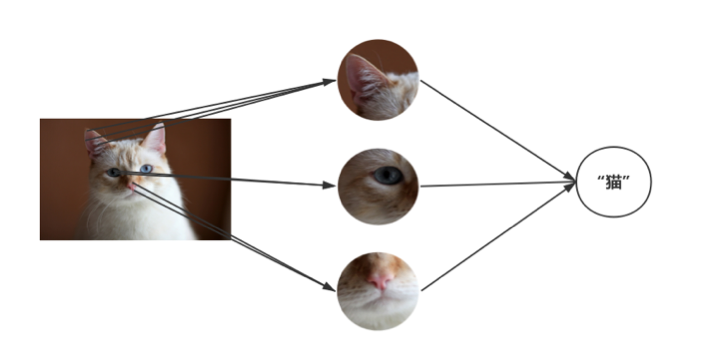
\includegraphics[width=0.6\textwidth]{cat1}
  \caption{视觉世界形成了视觉模块的空间层次结构:比如猫的超局部的边缘组成局部的对象, 比如眼镜或耳朵, 这些局部对象又组合成高级概念“猫”.\label{fig:cat1}}
\end{figure}

\normalsize
卷积的工作原理是在图像上滑动一个$3\times 3$的窗口, 它在每个位置停止并提取该位置的所有像素点, 构成一个多维矩阵. 然后将其同一个权重矩阵 (卷积核) 做张量积, 转化为以为一维的向量. 然后将这些向量组合起来转换为多维的输出图像. 详细过程如 \figref{fig:conv1} 所示, 本文将使用Keras的Conv2D来完成这一工作. 
\begin{figure}[hbtp]
	\centering
  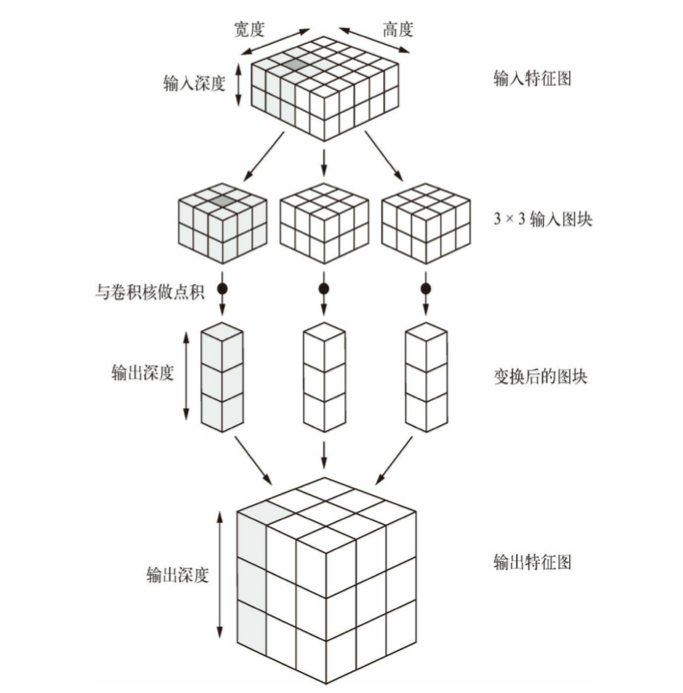
\includegraphics[width=0.5\textwidth]{conv1.png}
  \caption{卷积的工作原理.\label{fig:conv1}}
\end{figure}

\subsubsection*{池化层}
池化层的输入就是卷积层输出的原数据与相应的卷积核相乘后的输出矩阵. 池化层的目的是: 
\begin{enumerate}
	\item 减少训练参数的数量, 降低卷积层输出数据的维度; 
	\item 减小过拟合现象, 只保留最有用的图片信息, 减少噪声的传递; 
\end{enumerate}

本文使用的是MaxPooling2D从输入的数据中提取最大值, 然后输出. 
\subsubsection*{全连接层}
全连接层的每一个结点都与上一层的所有结点相连, 它起着将已经提取到的特征综合起来的作用. 而全连接层和卷积层的根本区别在于全连接层从输入特征空间中学到的是全局模式, 卷积层学到的是局部模式. 卷积层和池化层的工作就是提取特征, 减少原始图像带来的参数. 在本文中, 为了生成最终的输出, 需要应用全连接层来生成分类器. 全连接层的存在大大减少特征位置对分类的影响. 
\begin{figure}[hbtp]
\centering
  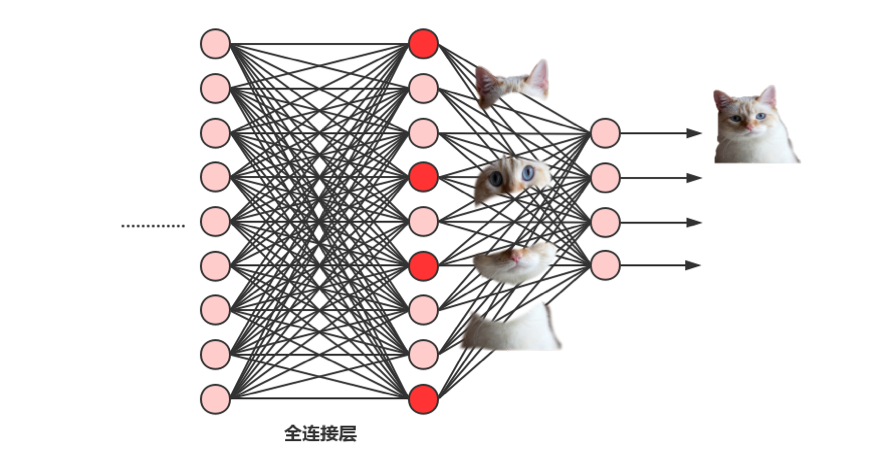
\includegraphics[width=0.7\textwidth]{densecat.png}
  \tiny
  \caption{图中正红色的神经元表示特征被激活了, 同一层的其他神经元, 要么猫的特征不明显, 要么未被发现. 当我们把这些特征组合在一起, 即为猫. \label{fig:densecat1}}
\end{figure}
\normalsize
\subsection{VGG模型}
在文章的第二部分, 使用了预训练的VGG19模型来进行迁移学习. 


\subsection{网络构建}

首先, 我们自建了一个小型的卷积神经网络, 并对其进行训练, 其网络结构如 \figref{fig:cnn1} 所示. 
\begin{figure}[hbtp]
	\centering
	  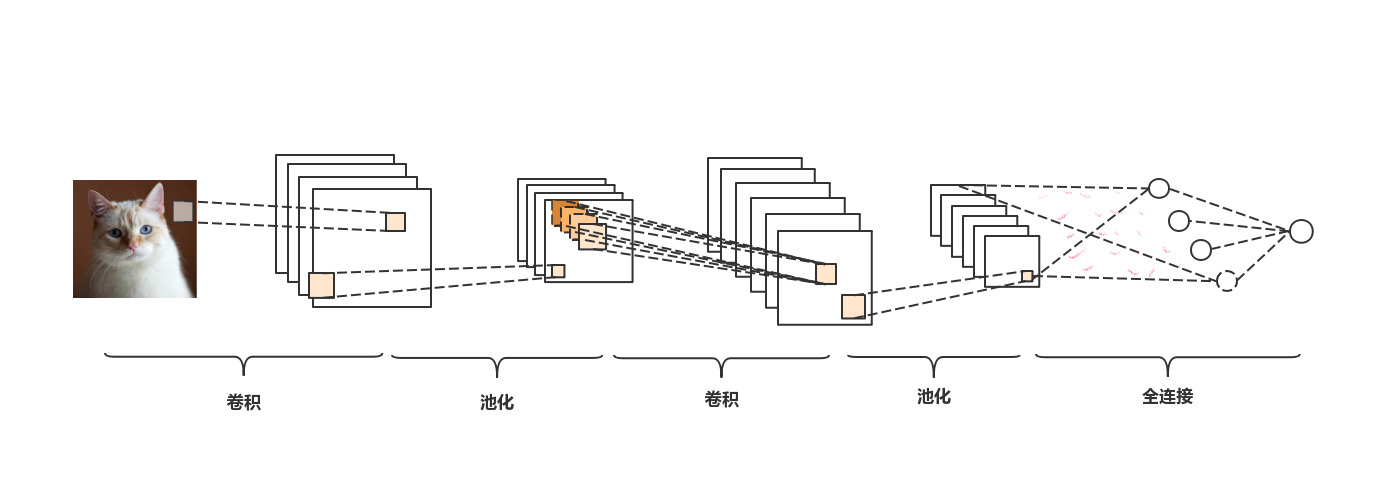
\includegraphics[width=0.85\textwidth]{cnn1.png}
	  \tiny
	  \caption{小型CNN结构示意.\label{fig:cnn1}}
\end{figure}
\normalsize
此CNN由Conv2D (使用relu激活) 和MaxPooling2D层交替堆叠构成. 这里我们使用4个Conv2D + MaxPooling的组合来增大网络容量, 也进一步减小特征图的尺寸, 使其在连接层Flatten层时尺寸不会太大. 由于我们面对的是一个二分类问题, 所以网络的最后一层是使用sigmoid激活的单一单元, 使用二元交叉熵作为损失函数. 

其次, 我们还使用VGG19进行了迁移学习, 直接将数据输入VGG19的卷积基部分, 然后在其顶部添加Flatten层和Dense层进行输出. 

\section{模型的训练}

在多次尝试使用配置机器失败后, 我们选用了一台配备了i7-8700K与单卡GTX1080Ti的机器(keras 2.2.4, tensorflow 1.4.1)上进行了我们简单模型的实验. 因为在算力上的短板, 使得我们的模型在全数据上的训练时间过长, 因此, 不得不在实验的数据量与网络大小上妥协. 但是在此基础上我们对模型进行了的几次改进, 依旧取得了不错的成果. 

\subsection{数据收集与处理}
本文使用Kaggle上的猫狗分类数据集, 这个数据集(training的部分)包含25000张猫狗图像 (两个类别都有12500张) . 我们将其两类分别随机分出了1000张作为训练集, 各500张作为验证集 500张作为测试集数目.

  数据预处理的步骤大致如下:

\begin{enumerate}
	\item 读取图像文件.
	\item 将JPEG文件解码为RGB像素网格($150\times 150$)
	\item 将这些像素网格转换为浮点数张量
	\item 将像素值 (0-255) 缩放到[0,1]区间
\end{enumerate}
我们调用了Keras的preprocess.image类里的ImageDataGenerator来完成这项工作. 同时, 整个数据集被分成了20个batch, 每一个batch有100个样本. 

\subsection{自建CNN训练}
首先, 我们对于自建的神经网络在数据及上进行了训练, 损失函数为交叉熵, 优化算法为RMSprop, 学习率为1e-4, 得到的结果为
\begin{figure}[hbt]
	\centering
	  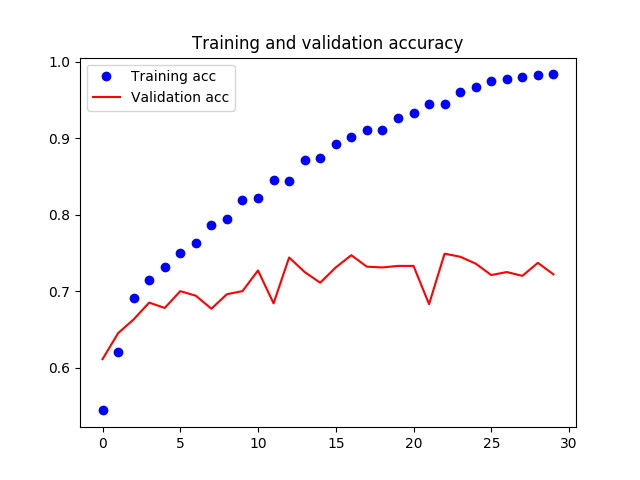
\includegraphics[width=0.45\textwidth]{small_without_aug_1}
	  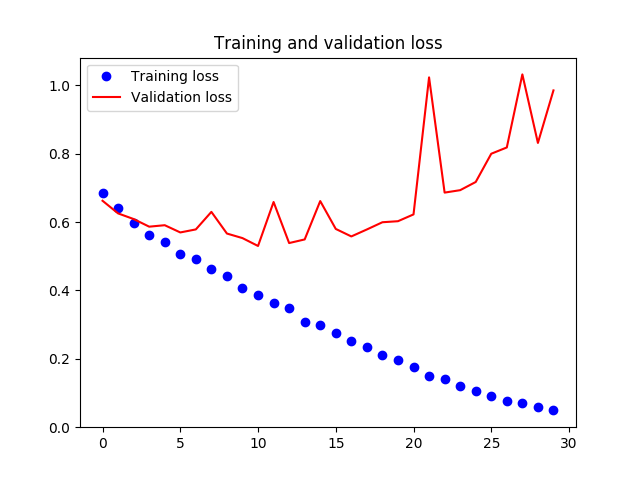
\includegraphics[width=0.45\textwidth]{small_without_aug_2}
	  \caption{自建网络训练结果.}
\end{figure}
此模型的准确度约为73.3\%, 并不是十分的高, 由于网络并不是很大, 训练速度也十分的快. 
\subsection{改进实验细节}

因为算力的短板, 我们另寻他路. 希望能够尽量提高在这样的算力所允许自由实验的前提下达到最好的结果. 我们从第一次试验的结果里可以发现我们的问题主要是算力能够驱动的数据量太小导致了过拟合. 于是我们便引入了数据增强与预训练模型VGG19来进行改进. 并且我们在试验后期又加入了两块新的GPU, 使得我们能够从容地对VGG19的最后段的卷积进行解锁训练, 进一步地提升了性能. 同时我们又测试了VGG16的性能, 发现VGG19比VGG16的表现强大约1\%. 




\subsubsection{数据增强避免过拟合}
由于我们的限制, 能够调用的学习样本并不算多,可能会出现过拟合的情况,所以我们采用数据增强的方法,利用多种能够生成可信图像的随机变换来增加样本,增强泛化能力。 在Keras中,可以利用ImageDataGenerator读取的图像进行多次随机变化,其中的随机变换由多个参数控制,如角度、缩放的范围、平移范围等, 从而生成更多的样本达到抗过拟合的效果, 如 \figref{fig:augcat}.
\begin{figure}[hbtp]
\centering
  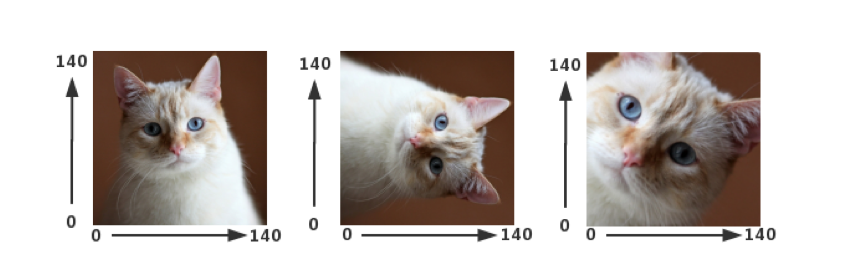
\includegraphics{aug.png}
  \caption{通过随机数据增强生成的猫图像\label{fig:augcat}}
\end{figure}

其中, 数据增强的变换参数设置为, 随机40度的旋转角, 随机20\%的平移, 随机20\%的放大缩小, 随机20\%的斜向拉伸并允许翻转的条件下, 损失函数为交叉熵, 优化算法为RMSprop, 学习率为1e-5, 此次改进后, 训练结果如下
\begin{figure}[hbt]
\centering
  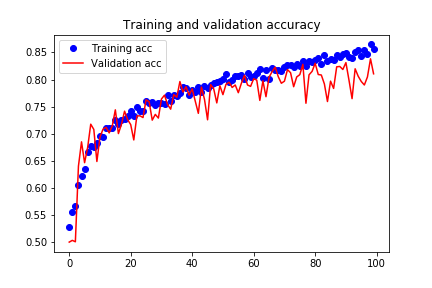
\includegraphics[width=0.45\textwidth]{small_aug_1.png}
  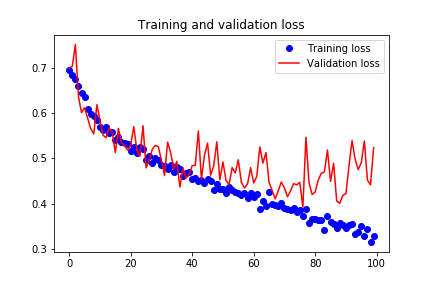
\includegraphics[width=0.45\textwidth]{small_aug_2.png}
  \caption{迁移学习训练结果}
\end{figure}
实现了在测试集上81.8\%的准确率. 表现不错但是依然不尽如人意.

\subsubsection{引入预训练模型VGG19}
由于自建的网络深度不够可能是准确率不高的主要原因, 我们考虑使用VGG19与训练模型来进行迁移学习. 

我们在VGG19预训练特征提取网络后面加上了两层全连接网络, 在训练集上进行了训练. 损失函数为交叉熵, 优化算法为RMSprop, 学习率为1e-5, 
\begin{figure}[hbt]
	\centering
	  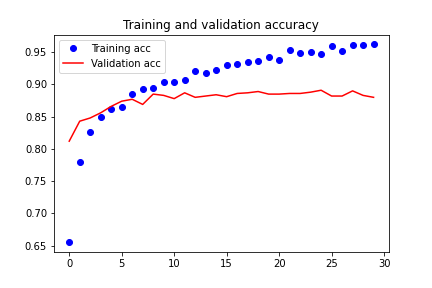
\includegraphics[width=0.45\textwidth]{VGG_classify_1}
	  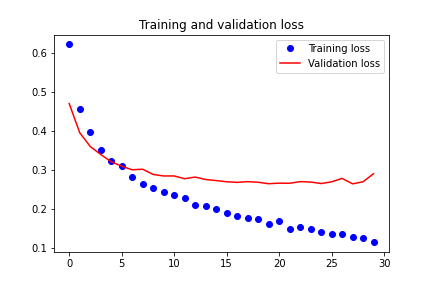
\includegraphics[width=0.45\textwidth]{VGG_classify_2}
	  \caption{带有数据增强的网络训练结果}
	\end{figure}
\subsubsection{VGG19后端解锁}

由于卷积神经网络卷积部分的特征提取功能从前段到后段有着逐渐抽象的特性. 前段负责物体的纹理边缘等低阶特征提取而后段负责对如位置关系这样的高阶抽象特征的提取, 我们可以期望对于我们这样一个阿猫阿狗数据集的低阶特征与其他数据集无异, 猫的边缘跟车的边缘, 猫的体表纹理跟狗的体表纹理不存在质的差距. 让猫是猫的不是猫这里有一条显著的边缘, 而是猫的这些边缘之间的关系. 所以对于在更大数据集上训练出来VGG19网络的前端的低阶特征提取的卷积, 我们可以认为它有着较好的泛化性. 但是对于后端的网络, 我们希望它的卷积在高阶特征上能够更多地去提取对猫狗分类这样一个问题有效的高阶特征. 于是我们解锁了后VGG19网络里的第五个卷积块的后四层卷积, 一层大约2,359,808个参数, 在我们的训练集上进行了训练. 并且为了避免过拟合, 我们还在网络训练过程中加入了Dropout.


%\begin{figure}[hbt]
%\centering
%  \includegraphics[width=0.45\textwidth]{}
%   \includegraphics[width=0.45\textwidth]{}
%  \caption{}
%\end{figure}

从图上可以看出因为我们的训练集在有了数据增强以后依然太小, 所以在训练VGG19的后端卷积层时依然出现了过拟合的现象

最后在测试集上达到了喜人的93.3\%的准确率.





\section{可视化}

我们最开始的打算是希望能够可视化整个模型训练过程中的特征图与滤波器的选择的变化, 让keras在自动化训练的每一个epoch的时候输出一次可视化结果. 但是因为这样的操作涉及更改Keras源码, 需要重写keras的训练函数, 在查看了Keras源码以后我们发现这个工作的工作量远远超出了我们的预计. 于是我们选择了一种相对简单但是也相当直观的可视化方式. 在模型训练完毕了以后对于模型的每一层的特征图与滤波器的滤波现象进行可视化.

在可视化VGG16与VGG19的滤波器的过程中, 我们的GTX1080Ti又遇到了算力不足完成一次试验需要太久的问题, 我们不得不再租用一台双卡Titan Xp进行试验, 在速度上得到了超过两倍的提升的同时很好地完成了可视化任务. 并且我们在可视化的过程中也发现了一些有趣的问题与现象.



\subsection{可视化中间输出}

我们对自建的简单模型所得到的卷积层进行了正向传播, 并希望在中间的每一步, 能够获得图像在经过这些滤波器作用后的输出. 我们调用了Keras的Model类来对我们的模型进行分步的实例化实现这一操作.

原图为: 
\begin{figure}[hbtp]
	\centering
	  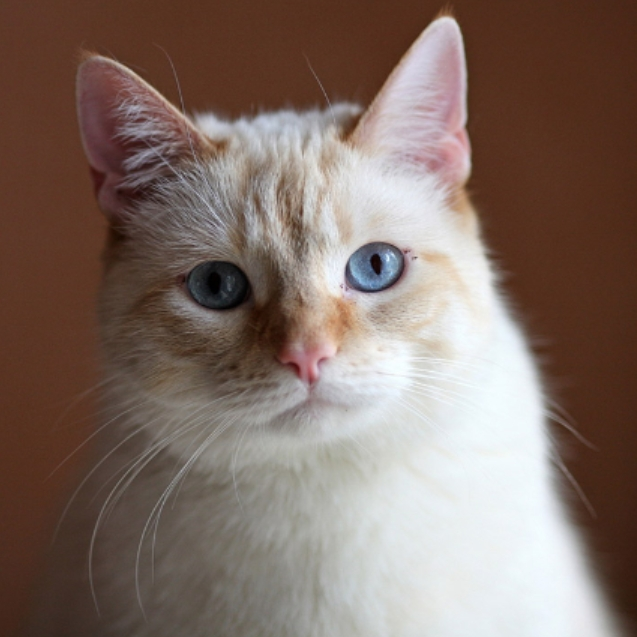
\includegraphics[width=0.3\textwidth]{a.jpg}
	  \caption{原本图像.}
\end{figure}

得到的几个中间输出结果为
\begin{figure}[hbtp]
\centering
  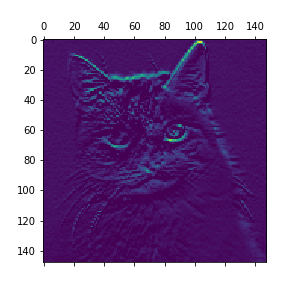
\includegraphics[width=0.30\textwidth]{30.png}
  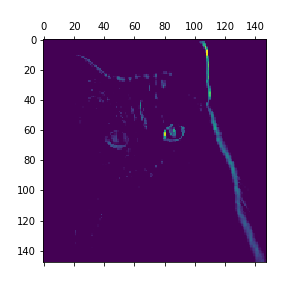
\includegraphics[width=0.30\textwidth]{25}
  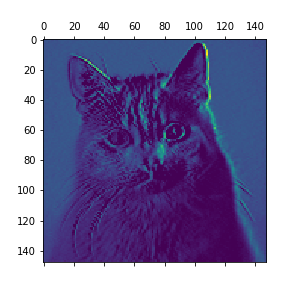
\includegraphics[width=0.30\textwidth]{15}
  \caption{左为第30个滤波器, 中为第25个滤波器, 右为第15个滤波器.}
\end{figure}

通过对比其这一层所有滤波器的结构我们发现所有的滤波器都应该学习到了不同的特征. 我们还对后面的所有卷积层与池化层都进行了这样的可视化, 希望能够了解机器是如何理解从低阶到高阶的特征的, 如下图所示. 

\begin{figure}[h]
\centering
  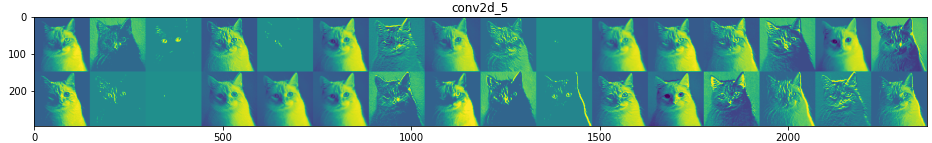
\includegraphics[width=1\textwidth]{conv2d_5.png}
\end{figure}
\begin{figure}[h]
	\centering
  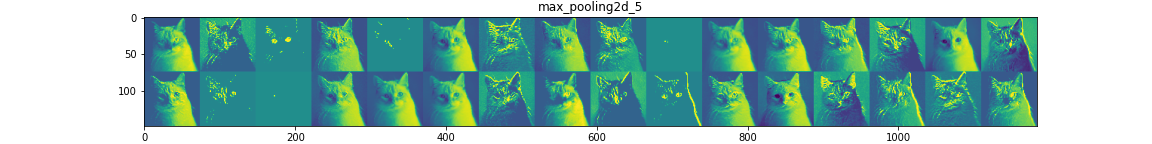
\includegraphics[width=1\textwidth]{max_pooling2d_5}
\end{figure}
\begin{figure}[h]
	\centering
  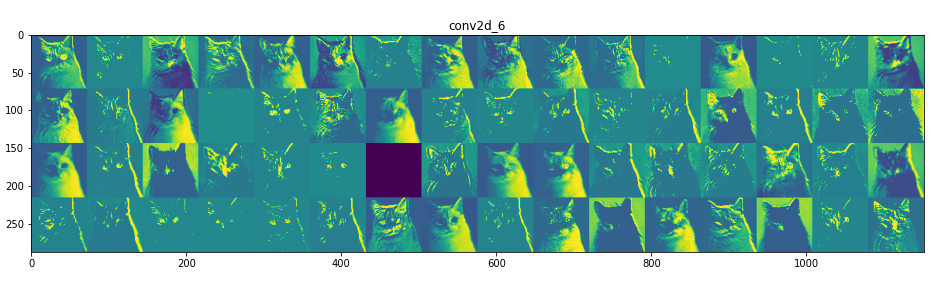
\includegraphics[width=1\textwidth]{conv2d_6}
\end{figure}
\begin{figure}[h]
	\centering
  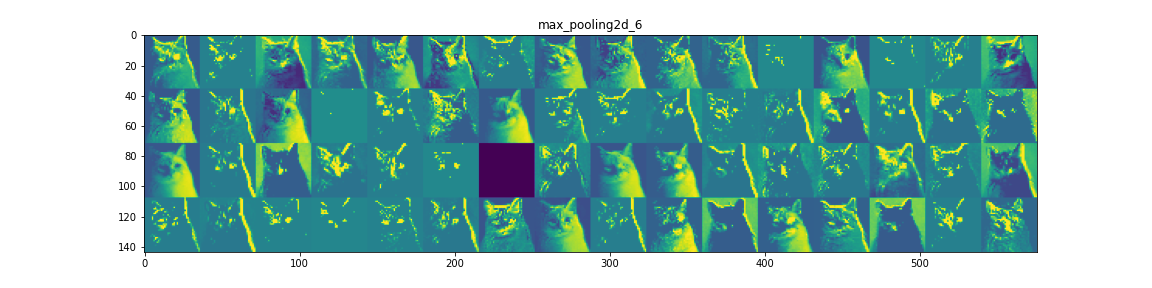
\includegraphics[width=1\textwidth]{max_pooling2d_6}
\caption{第五、六层卷积层与池化层前向传播的可视化.}
\end{figure}
\begin{figure}[hbtp]
	\centering
  
  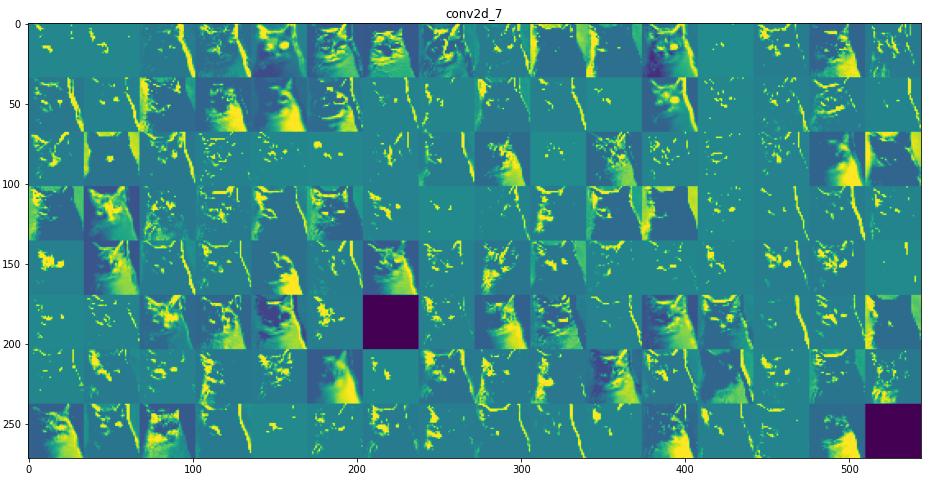
\includegraphics[width=0.75\textwidth]{conv2d_7}\\
  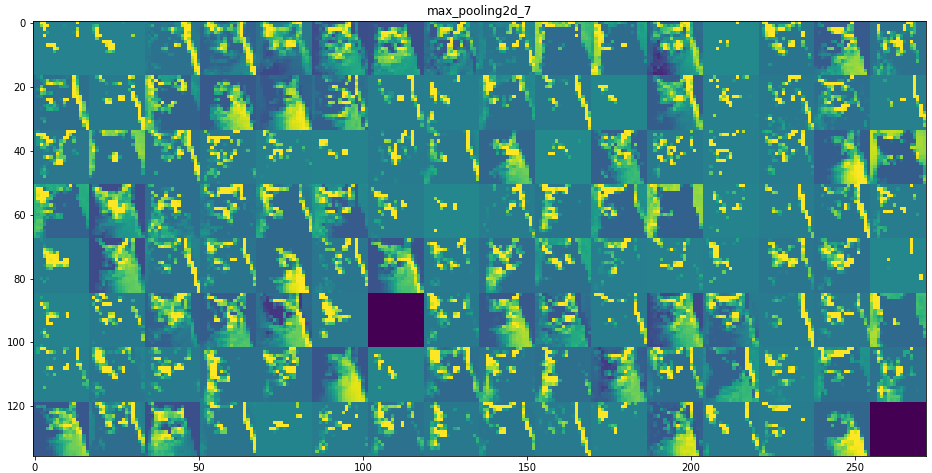
\includegraphics[width=0.75\textwidth]{max_pooling2d_7}\\
  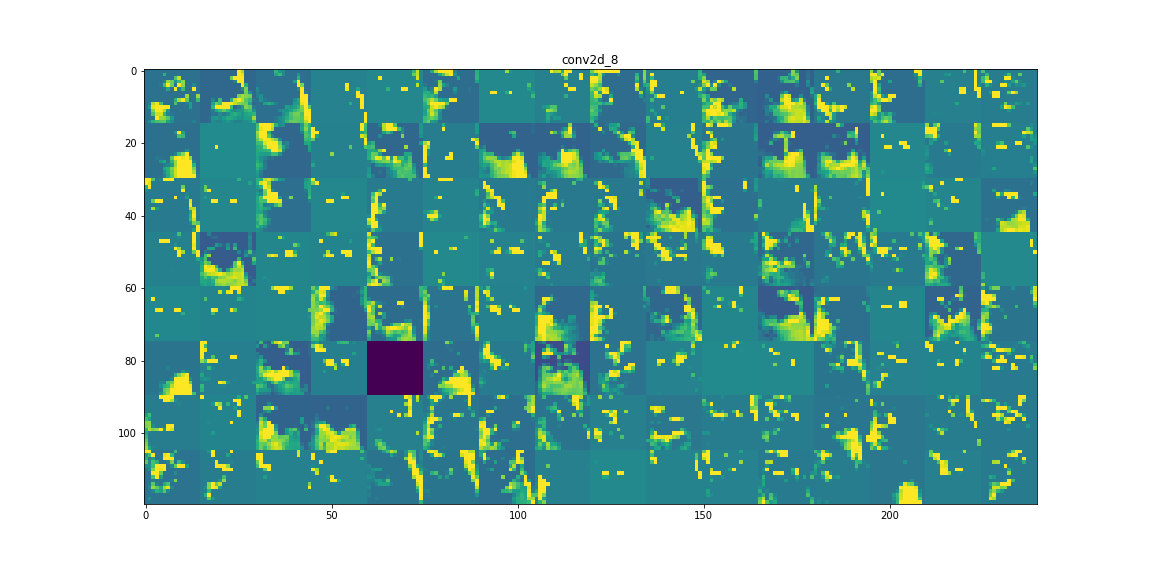
\includegraphics[width=0.75\textwidth]{conv2d_8}\\
  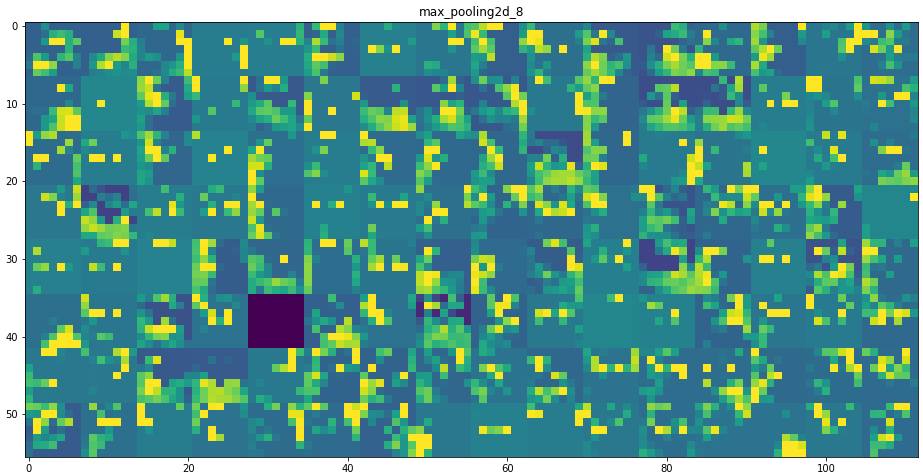
\includegraphics[width=0.75\textwidth]{max_pooling2d_8}
  \caption{从第五层到第八层的卷积层与池化层的前向传播可视化\label{fig:forward1}}
\end{figure}

从\figref{fig:forward1}中可以看出随着卷积层的深入, 滤波器所得到的激活值所可视化出来的图像的可读性在逐渐降低, 浅层的图像还是能看到猫的轮廓与明显的猫的特征, 但是随着网络的深入我们就逐渐无法描述或是理解这些示波器是如何处理这些图像的了.







\subsection{可视化过滤器}

我们希望可视化的是滤波器(卷积部分+ReLu)部分的的功能, 换句话说, 我们希望可视化的是这样的滤波器提取出来的是什么特征. 为了做到这一点, 我们需要知道这样的滤波器$f_0$在什么样的输入$X$下给出最大的输出值$Y$, 即我们需要在输入空间$\mathcal X$里得到$\arg \max_{X\in \mathcal X} f_0(X)$. 那么我们如果能引入一个度量使得最大化$f_0(X)$等价于最大化这个度量, 我们就可以在输入空间$\mathcal X$上梯度下降来进行优化. 我们取这个度量为网络输出张量的所有坐标的均值. 从一张带有微弱噪声的灰色的(RBG各值在每个坐标上均为128, 加上了一个从均匀随机的噪声$\sigma\in[0,20]$)的图像开始, 调用了Keras后端的Tensorflow里的随机梯度下降函数来进行实现. 并且在对输入空间即图像更新时, 我们采用了归一化的技巧使得我们的更新能够更加稳定. 在第一次尝试可视化的过程中, 我们的训练过程因数值上溢终止, 于是我们在归一化的同时还给里面加入了一个常数1e-5来避免这样的现象. 通过对五个卷积模块的第一个filter进行了40步的随机梯度下降, 再一次对图像张量进行归一化处理将其颜色坐标转换到[0,1]区间上, 通过调用plt.imshow()函数, 我们终于得到了VGG的filter的第一个可视化图像. 

\begin{figure}[hbtp]
  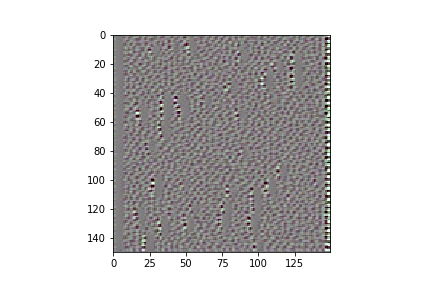
\includegraphics{block2_conv1_127.png}
  \caption{预训练的VGG19网络第二个卷积模块的第一个卷积层的第127个滤波器所在识别的图案可视化图.\label{fig:pretrain-singal}}
\end{figure}


但是当我们尝试讲所有滤波器的图像都进行可视化的时候我们也发现了一些我们没有想到的有趣现象.

\begin{figure}[hbtp]
\centering
  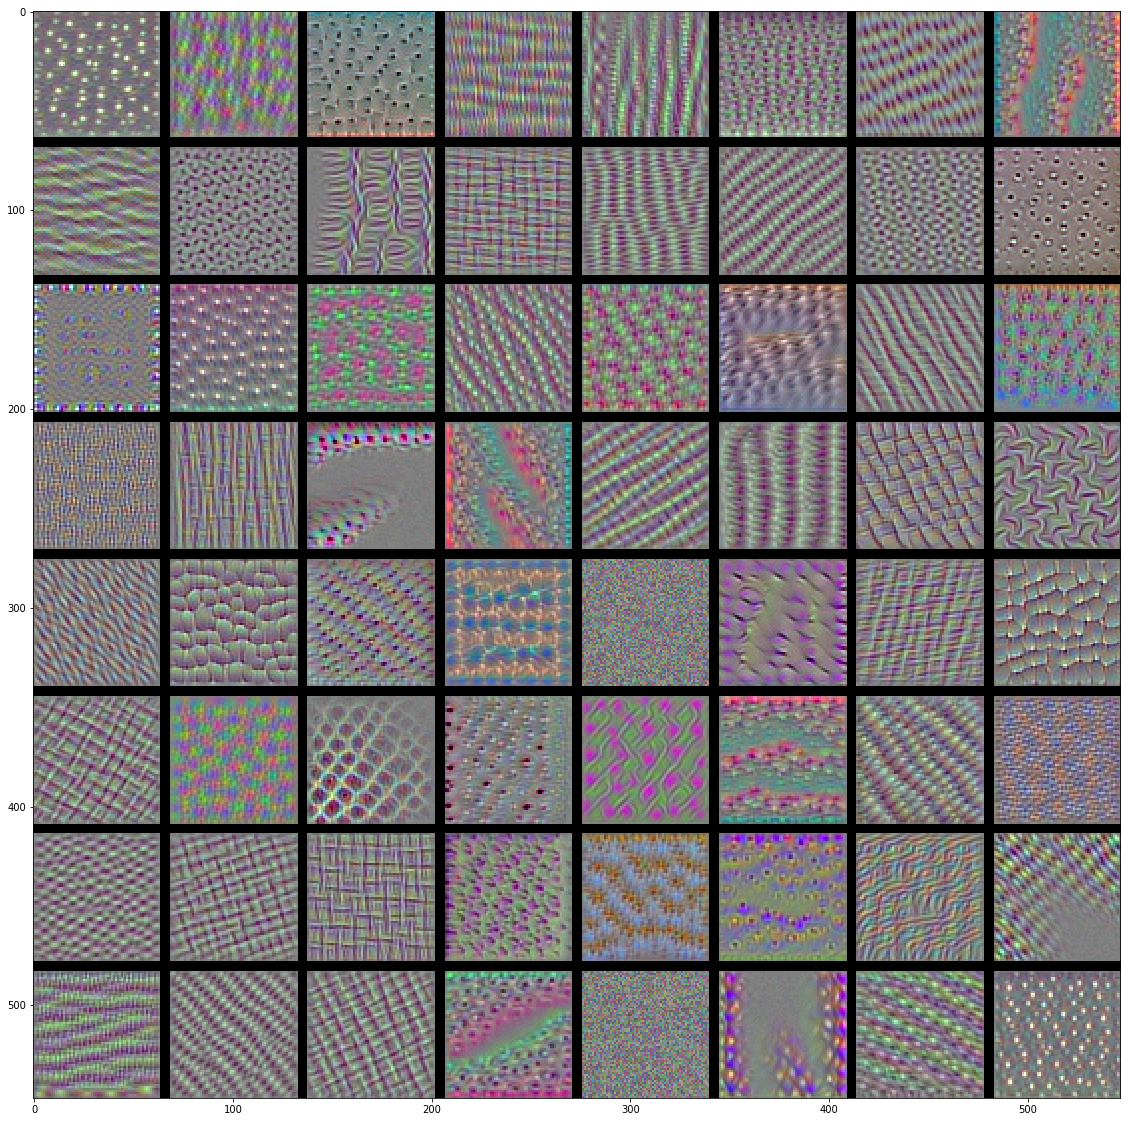
\includegraphics[width=0.8\linewidth]{block3_conv1}
  \caption{预训练的VGG19网络第三个卷积模块的第一个卷积层中的64个滤波器识别的图案的可视化图\label{fig:filter3}}
\end{figure}



\begin{figure}[hbtp]
\centering
  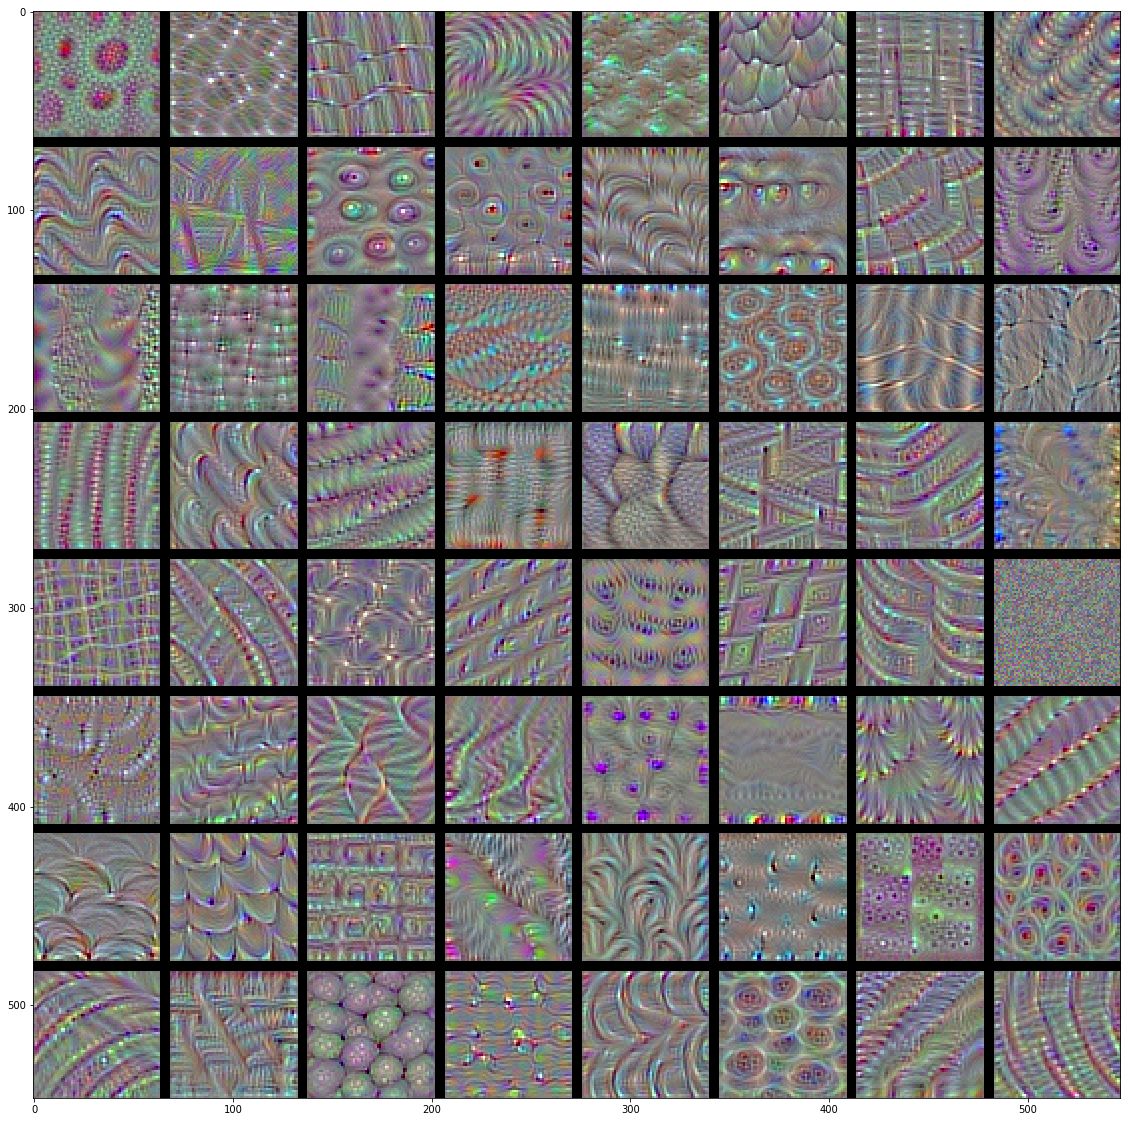
\includegraphics[width=0.8\linewidth]{block4_conv1}
  \caption{预训练的VGG19网络第四个卷积模块的第一个卷积层中的64个滤波器所识别的图案可视化图\label{fig:filter4}}
\end{figure}

\begin{figure}[hbtp]
\centering
  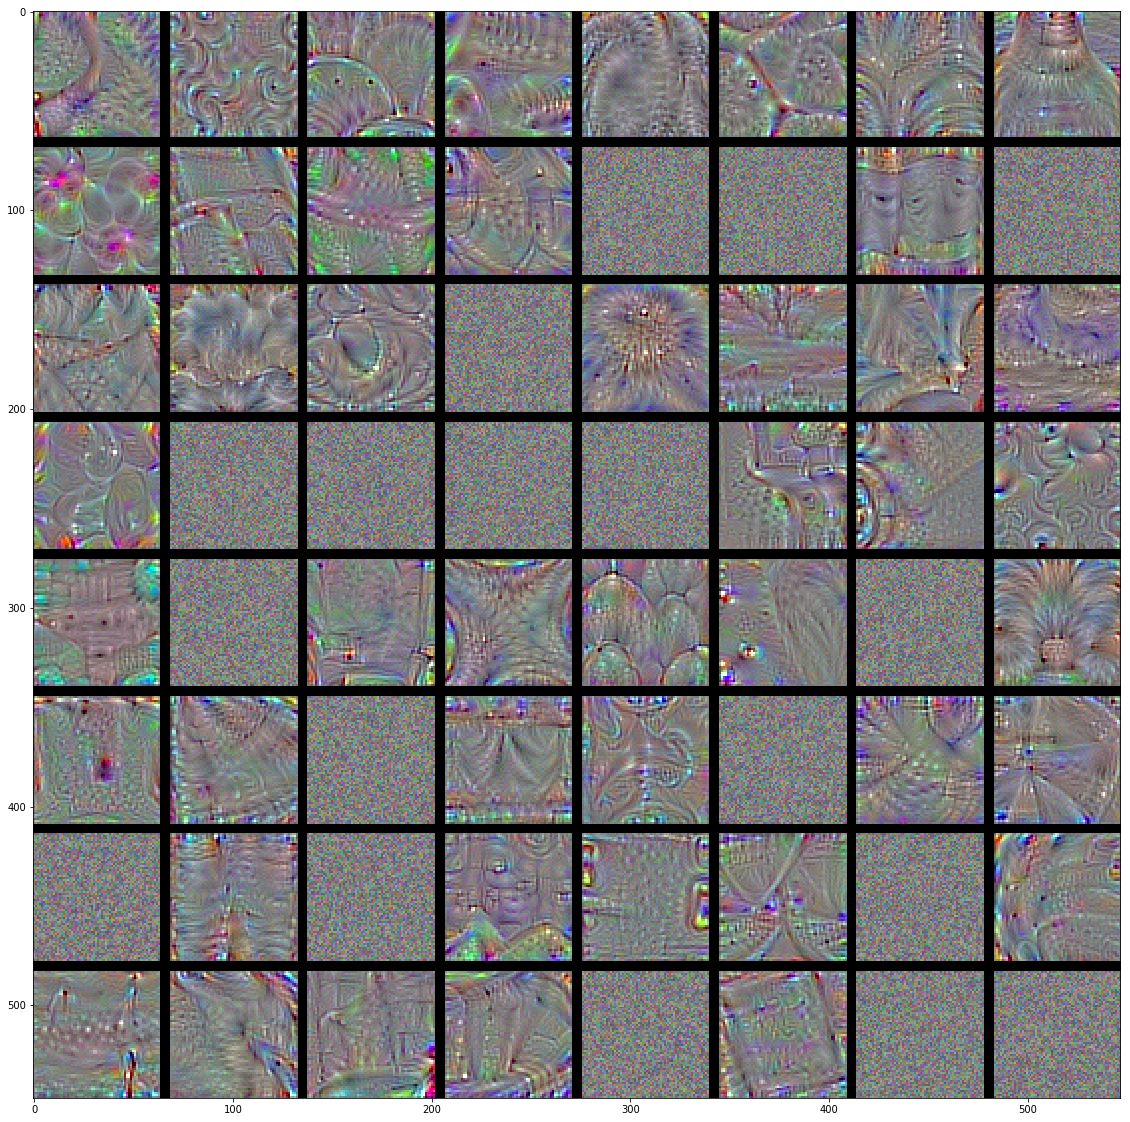
\includegraphics[width=0.8\linewidth]{block5_conv1.png}
  \caption{预训练的VGG19网络第五个卷积模块的第一个卷积层中的64个滤波器识别的图案的可视化图\label{fig:filter5}}
\end{figure}

通过观察我们可以发现从第三个卷积模块开始\figref{fig:filter3}, 我们的滤波器所识别的图像可视化出来的结果出现了完全是噪声的图像. 并且随着卷积网络的深入, 这样的全部是噪声的图像的数目在不断增加\figref{fig:filter4}, 到了第五个卷积模块\figref{fig:filter5}, 一半的滤波器可视化出来都是与初始噪声相同的模样. 换句话说有可能这些滤波器在输入空间中没有作用, 这个时候随着网络的深入它所探测的特征已经超出了我们的人眼能够分辨的明显的特征, 又或者是随机梯度下降无法很好的还原这些高阶的巨大的卷积块的偏好? 我们无法给出这样的现象的解释.

%\begin{equation}
%	\begin{aligned}
%		x = \arg \min \text{mean}(f_0(X))
%	\end{aligned}
%\end{equation}





\newpage
\nocite{*}

% 如果想修改参考文献样式( 非国标 ), 请把下行取消注释, 并换成合适的样式( 比如 unsrt, plain 样式 ). 
\bibliographystyle{unsrt}
\bibliography{wpref}

\end{document}
